\documentclass[runningheads]{llncs}
\usepackage[T1]{fontenc}
\usepackage{lmodern,microtype,amsmath,amssymb,graphicx,booktabs,tabularx}
\setlength{\emergencystretch}{1.5em}
\usepackage[hidelinks]{hyperref}
\graphicspath{{assets/}}
\begin{document}
\title{EvidencePath Companion S1}
\titlerunning{EvidencePath Companion S1}
\author{Anonymous Authors}
\authorrunning{Anonymous Authors}
\institute{}
\maketitle

\paragraph{Role.} This companion provides procedures for review and archiving. The 16-page main paper is self-contained; separate supplementary submission is subject to venue rules.

\section{Models and reconstruction}

\paragraph{Graph retrieval and features.}
The graph branch combines direct targets, indications, and shared-pathway candidates. Only shared-pathway candidates require at least five common pathways and Jaccard overlap of at least \(0.08\), are sorted by decreasing Jaccard and profile-pathway coverage with canonical/raw names breaking ties, and are capped at 30. The complete union with direct-target and indication candidates may exceed 30; neither CIViC retrieval nor the final union receives this cap. The graph features encode targeting, \(\log(1+\mathrm{shared\ pathways})\), profile-pathway coverage, pathway Jaccard, and indication. For each CIViC level group, SF uses \(\log(1+\mathrm{count})\) of visible drug-level evidence pooled across contexts. Missing features are zero. Graph-pool membership and SF order therefore do not constitute controls free of clinical information.

\paragraph{Frozen models.}
July 2025 supervision includes 84 training pairs (31 queries) and 16 validation pairs (seven queries) with disjoint molecular profiles. Training features exclude each candidate's label-defining evidence items. Other items from the same publication can remain. Simple Fusion (SF) is a frozen eight-feature LightGBM LambdaMART model~\cite{lightgbm} with four trees, learning rate 0.05, seven leaves, depth at most three, minimum leaf size three, L2 penalty one, and seed 7147. Inputs are five graph features and three log-transformed CIViC grade counts (A/B, C, D/E). The frozen AltGraph model uses nine features including a graph-missing indicator, two ordinal gradient-boosted trees, and learning rate 0.05. Both rank by decreasing score, then ascending canonical drug name. The archived environment uses Windows 11, Python 3.12.13, and LightGBM 4.7.0.

\paragraph{Stored ranks and source descriptions.}
Reconstruction matches B0--B6 over 1,051 January candidates. The corrected quarterly matrix adds 1,711 candidates after excluding four ineligible combinations. Rebuilding with the archived P4 descriptors reproduces all 105 affected candidate entries, memberships, and B0--B6 ranks across three replay queries and one cutoff-defined query. A rerun uses the source descriptions with fixed snapshots, mappings, eligibility rules, and models. Both descriptions yield empty validated-gene sets for two W1 queries. The source descriptions add AGAP3 for W3 MP:6036 and AGK for W3 MP:281. Branch memberships agree. Mix swaps unlabeled cetuximab and vemurafenib at ranks 49 and 50 for cutoff-defined MP:281. All four positives retain their ranks or unretrieved status. In both full quarterly cohorts, coverage, query and pair MRR, and HR@5 agree for Graph, Append-SF, AltAppend, RRF, Context, and both insertions.

\paragraph{Constrained insertion.}
Both policies preserve the graph order \(O=(o_i)\) and a fixed addition order \(N'=(n_j)\). Original insertion orders additions by decreasing \(v\) and SF score, then ascending name. Evidence insertion uses the CIViC order. Priority is \(v=(a-1)/(|R_1|-1)\), where \(a\) ranks \((b,m,c,h,\ell,n)\) from weak to strong across \(R_1\) with average ranks for ties. If \(b<2\) and \(n=0\), use the SF rank computed separately across \(R_1\) with the same tie rule. Singletons receive \(v=1\). With \(D(r)=1/\log_2(1+r)\) and \(s=|O|\), dynamic programming maximizes
\[
  \sum_j v(n_j)\,[D(r_L(n_j))-D(s+j)]
  -\lambda\sum_i D(i)\,[D(i)-D(r_L(o_i))].
\]
Both policies use \(\lambda=4\), selected on January development. When two transitions differ by at most \(10^{-12}\), the solver ends the current prefix with an old item. The oracle preserving both fixed orders has MRR 0.3294. RRF exceeding this bound requires at least one constraint to be relaxed, without identifying which one. The oracle preserving only \(O\) while freely ordering additions reaches 0.4568, above RRF.

\section{Added fixed-pool diagnostics}

These E0--E6 analyses were performed after the original replay results were available. They are post hoc diagnostics, not a newly preregistered test or prospective clinical validation. No frozen model is retrained.

\paragraph{E0: reconstruction and units.}
The analysis bundle freezes candidate identities, labels, branch membership/ranks, and deterministic tie rules. It contains 1,580 union candidates, 45 queries, and 46 positive pairs for main replay; the three cutoff-defined pairs remain separate. Query keys include the replay window. Query reciprocal rank is that of the first eligible positive, with zero when none is retrieved, and HR@\(k\) is a query-level indicator. Pair statistics and pair-level top-five counts use explicitly separate denominators. Exact rational RRF~\cite{rrf}, with the frozen \(k=60\), equal weights, and specified final tie rule, reconstructs every stored RRF candidate rank. Before/after hashes confirm that all 39 registered inputs remain unchanged.

\paragraph{E1: paired dependence-aware uncertainty.}
The primary comparator is Context on the identical candidate union. RRF's replay MRR difference is \(+0.0435\), with 9/23/13 query wins/ties/losses. Separate connected-component partitions join queries sharing a positive drug or a canonical label-support source. They contain 19 drug clusters (largest seven queries) and 24 source clusters (largest six). Each partition uses 10,000 PCG64 bootstrap rounds, sampling \(C\) whole clusters with replacement from \(C\) and recomputing the query-weighted paired mean with the actual sampled query denominator. Drug/source seeds are 2026112301/2026112302; linear empirical percentiles define the 95\% intervals.

RRF--Context intervals are \([-0.0692,+0.1718]\) and \([-0.0652,+0.1666]\), both spanning zero. These limited-sample comparisons do not establish equivalence. The same draws support the secondary CIViC comparison, which has a different candidate pool. Leave-one-cluster-out RRF--Context gaps remain positive (approximately 0.0097--0.0802), describing influence within the observed sample rather than overriding bootstrap uncertainty. Neither partition captures every possible dependence relation.

\paragraph{E2: membership and depth.}
Shared-first stably partitions the complete Context ranking into candidates in both branches followed by candidates in only one, preserving Context order within either group. It has no fitted score, but its inspection here is post hoc. Replay MRR is 0.4265 versus RRF's 0.3895, whereas development MRR is 0.3750 versus RRF's 0.4594. This reversal does not validate Shared-first as a replacement. Sequential differences among CIViC, Context, Shared-first, and RRF alter several properties and are not an additive causal decomposition.

Table~\ref{tab:lengths} includes empty lists in each cohort's complete branch-length distribution. Table~\ref{tab:tradeoff} uses positive-pair denominators: 13 evidence-exclusive replay positives and ten positive pairs in Append-SF's original top five. It exposes a depth-dependent exchange between finding additions and retaining early old positives; these are not the query-level HR@5 denominators.
% Generated from frozen artifacts; edit build_revision_tables.py, not numeric cells.
\begin{table}[t]
\centering
\caption{Branch lengths}
\label{tab:lengths}
\small
\setlength{\tabcolsep}{3.5pt}
\begin{tabular}{llrrr}
\toprule
Cohort & Branch & Median & Range & Empty \\
\midrule
Development & CIViC & 7 & 0--19 & 4 \\
Development & Graph & 12 & 0--50 & 4 \\
Replay & CIViC & 8 & 0--36 & 2 \\
Replay & Graph & 30 & 0--50 & 1 \\
\bottomrule
\end{tabular}
\end{table}

% Generated from frozen artifacts; edit build_revision_tables.py, not numeric cells.
\begin{table}[t]
\centering
\caption{Positive retention}
\label{tab:tradeoff}
\small
\setlength{\tabcolsep}{3.5pt}
\begin{tabular}{lrr}
\toprule
Policy & Evidence-only top five & Old top-five retained \\
\midrule
Context & 11/13 & 7/10 \\
RRF & 8/13 & 10/10 \\
Shared-first & 9/13 & 9/10 \\
\bottomrule
\end{tabular}
\end{table}


\paragraph{E3: conditional order shuffles.}
The graph-order control independently permutes each query's full graph list within each of 5,000 PCG64 rounds, resetting seed 7147 in each cohort. Membership, the complete CIViC order, union, RRF parameters, and final tie rule stay fixed; exact one- or two-branch rational scores are recomputed. The full CIViC order includes SF as its terminal key, retaining that source of graph-related information. Archived CIViC-order draws are reused with hashes, while graph-order draws are newly computed. These controls perturb ordering, not membership or all information originating from a branch.

Table~\ref{tab:supp-shuffle} reports all 12 cohort/branch/metric tests; HR entries are percentages. The upper-tail test is \((b+1)/(5000+1)\), where \(b\) counts draws at least as large as observed; Holm correction covers the full 12-test family. Only replay CIViC-order HR@5 meets adjusted \(0.05\) (\(18/5001=0.0036\) raw, 0.0432 adjusted). Development graph-order MRR also exceeds its central 95\% shuffle range, but has adjusted \(p=0.0550\). Central ranges describe conditional permutation distributions, not confidence intervals for new-query performance. Tail counts, full distribution ranges and round-level metrics remain in the accompanying CSVs. Other non-rejections do not establish absence of graph information or quantify causal source contributions.
% Generated from frozen artifacts; edit build_revision_tables.py, not numeric cells.
\begin{table}[t]
\centering
\caption{Order shuffles across cohorts}
\label{tab:supp-shuffle}
\small
\setlength{\tabcolsep}{2.2pt}
\begin{tabular}{llrrrrr}
\toprule
Shuffled & Metric & Observed & Mean & Central 95\% & Upper $p$ & Holm $p$ \\
\midrule
\multicolumn{7}{l}{\textit{Development}} \\
Graph & MRR & 0.4594 & 0.4006 & $[\,0.3578,\,0.4465\,]$ & 0.0050 & 0.0550 \\
Graph & HR@3 (\%) & 48.78 & 48.09 & $[\,43.90,\,51.22\,]$ & 0.6079 & 1.0000 \\
Graph & HR@5 (\%) & 53.66 & 51.96 & $[\,48.78,\,53.66\,]$ & 0.4193 & 1.0000 \\
CIViC & MRR & 0.4594 & 0.4461 & $[\,0.4132,\,0.4799\,]$ & 0.2220 & 1.0000 \\
CIViC & HR@3 (\%) & 48.78 & 48.27 & $[\,43.90,\,51.22\,]$ & 0.6445 & 1.0000 \\
CIViC & HR@5 (\%) & 53.66 & 50.72 & $[\,48.78,\,53.66\,]$ & 0.0876 & 0.6131 \\
\midrule
\multicolumn{7}{l}{\textit{Replay}} \\
Graph & MRR & 0.3895 & 0.3433 & $[\,0.2974,\,0.3929\,]$ & 0.0324 & 0.2915 \\
Graph & HR@3 (\%) & 46.67 & 37.59 & $[\,31.11,\,44.44\,]$ & 0.0074 & 0.0740 \\
Graph & HR@5 (\%) & 60.00 & 57.07 & $[\,53.33,\,60.00\,]$ & 0.2044 & 1.0000 \\
CIViC & MRR & 0.3895 & 0.3514 & $[\,0.3085,\,0.3969\,]$ & 0.0498 & 0.3983 \\
CIViC & HR@3 (\%) & 46.67 & 42.82 & $[\,35.56,\,48.89\,]$ & 0.2134 & 1.0000 \\
CIViC & HR@5 (\%) & 60.00 & 50.85 & $[\,46.67,\,55.56\,]$ & 0.0036 & 0.0432 \\
\bottomrule
\end{tabular}
\end{table}


\paragraph{E4: actual-use source audit.}
For each query \(q\), input sources \(I(q)\) are typed, canonical publication identifiers from cutoff-visible evidence actually consumed anywhere in clinical retrieval/context ordering or SF evidence-count features. They include unsuccessful candidates, rather than only eventual positive hits. Label sources comprise all eligible support sources for each frozen positive pair. Evidence-item identifiers remain distinct from publication identifiers. Reconstruction uses the applicable cutoff and frozen positive set; it adds neither pilot nor later-created labels.

The audit reconstructs 11,171 query-used evidence records, resolves all source identifiers, and checks all 46 frozen replay pairs. Seven of 46 positives (15.2\%) across six queries share a label-support source with actual query input. Removing these labels while preserving every candidate rank leaves 39 queries and 39 positive pairs. RRF retains a higher MRR point estimate than Context/CIViC, but has 22 top-five hit queries versus 23 for either comparator. This sensitivity analysis does not establish publication independence or zero leakage. Same-source support need not invalidate a label, and absolute MRR changes across different label subsets are not themselves estimates of leakage.

\paragraph{E5: fixed-score coverage and displacement.}
Let \(g_q\) be the best reciprocal rank of an old positive in Graph, \(o_q\) that of old positives in expanded Mix, and \(m_q\) that of all positives in Mix, with zero for an empty set. The identity
\[
m_q-g_q=(o_q-g_q)+(m_q-o_q)
\]
separates old-positive displacement from the gain through added positives and averages over the same 45 queries. Graph-to-Mix pair coverage rises from 20/46 to 33/46 while MRR falls from 0.1902 to 0.1809: displacement is \(-0.030968\), the added-positive term \(+0.021714\), and the net \(-0.009254\). All 1,262 retained graph-candidate scores match the historical export; source inspection confirms one shared prediction vector for Graph and Mix. This verifies a fixed-score replay identity, not a separately trained model comparison or a general claim that expansion hurts.

\section{Retained sensitivity checks}

\paragraph{CIViC order shuffles.}
We use 5,000 PCG64 draws with seed 7147 in each cohort. The original replay order raises mean pair reciprocal rank by 0.0517 for shared positives and 0.0560 for CIViC-exclusive positives relative to the shuffle mean.

\paragraph{Ties.}
The replay audit reproduces all 438 CIViC branch ranks. Thirty-one queries contain ties on the first six keys. Using canonical drug name in place of SF to resolve those ties changes 82 ranks across 21 of 45 queries. A separate January check fixes branch ranks and takes the expectation over uniform orders within exact final-score tie blocks. The RRF--AltAppend MRR gap changes from 0.0448 to 0.0571, and RRF's expected top-five hit count remains 22.

\paragraph{Cutoff conflicts.}
Among the 221 RRF top-five replay positions, 21 carry the cutoff benefit-conflict flag. Each flagged position lacks an opposing record matching both the exact profile and exact disease. Eleven of the 46 eligible replay positives carry the flag, including eight of the 27 positives in the top five. For W3 ivosidenib, level-A benefit EID 7278 in acute myeloid leukemia and level-C anti-benefit EID 5987 in pancreatic cancer have the same shared-gene rank. The opposition triggers the ranking flag, while endpoint EID 12903 meets eligibility.

\paragraph{Historical development dependence.}
This RRF--AltAppend analysis is separate from E1's replay comparison against Context. Development clusters are connected components defined by shared positive drugs or canonical evidence sources. In each partition, the paired bootstrap draws whole clusters 2,000 times with seed 7147 and recomputes the query denominator in each replicate. The largest component has 14 queries in each partition. The RRF--AltAppend MRR gap is $+0.0448$. The 95\% percentile intervals are $[+0.0102,+0.1099]$ for 17 drug clusters and $[+0.0108,+0.1095]$ for 18 source clusters. The 35 leave-one-cluster comparisons give gaps of 0.0251--0.0540. These intervals do not transfer to the stronger Context comparison.

\paragraph{Matched omissions.}
Dropping W1, W2, or W3 retains 28, 39, or 23 replay queries, respectively. Dropping the largest shared-drug or recorded citation-ID component retains 38 or 39 queries. Across these five omissions, RRF's MRR gain ranges from 0.0130 to 0.1022 over the CIViC branch and from 0.1375 to 0.2062 over Append-SF. Its top-five hit-count difference with CIViC ranges from $-1$ to $+1$. Dropping the three replay queries affected by descriptor changes retains 42 queries and 43 pairs. The respective MRR gains are 0.0416 and 0.1763.

\section{Sealed pilot}
The September--October pilot sealed predictions before local receipt of the October snapshot. Both eligible pairs overlap W3 and are absent from the sealed lists. The counts of two positives and zero qualifying hard cases fell below the prespecified minima of ten and three. Verification requires the timestamped seal, pair ledger, and protocol. The pilot supplies no formal performance estimate and does not enlarge the 45-query replay denominator.

\section{E6: fusion parameters and reproduction}
\paragraph{Fusion weights.}
Figure~\ref{fig:s1-grid} varies \(k\in\{10,20,40,60,80,100\}\) and graph weight \(\alpha\in\{0.1,0.2,\ldots,0.9\}\), with evidence weight \(1-\alpha\). All 54 exact-rational settings fix pools, branch ranks, and tie policy and exceed Append-SF on query MRR in both cohorts. Against either Context or CIViC, however, replay has only 30 wins and 24 losses across the grid; development has 54 wins. The weak-baseline result therefore does not establish robust superiority over stronger comparators.

Red boxes in Fig.~\ref{fig:s1-grid} mark the frozen equal-weight \(k=60\) default, which remains unchanged. For the nine neighboring settings \(k\in\{40,60,80\}\), \(\alpha\in\{0.4,0.5,0.6\}\), replay MRR ranges from 0.3128 to 0.4279, HR@5 from 19 to 30 of 45, and the MRR difference from Context from \(-0.0332\) to \(+0.0819\). The archived heatmap shows absolute MRR, not confidence intervals, and does not establish superiority throughout the grid. Post hoc parameter selection on replay would introduce selection bias~\cite{cawley}.

\begin{figure}[!ht]
\centering
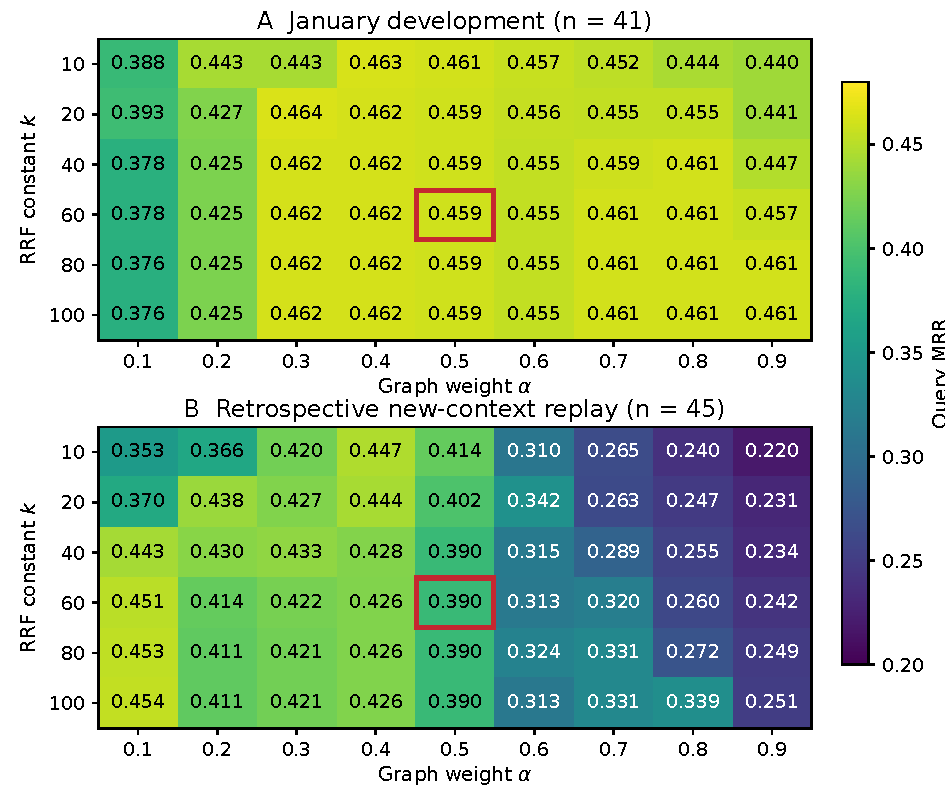
\includegraphics[width=.74\textwidth]{rrf_parameter_grid.pdf}
\caption{Parameter sensitivity}
\label{fig:s1-grid}
\end{figure}

\paragraph{Snapshot visibility.}
All 49 quarterly first observations cite PubMed records dated 2007--2025 and have evidence item identifiers (EIDs) absent at cutoff. An intermediate export shows accepted status for 31 EIDs. The same typed citation ID occurs somewhere in the opening cutoff snapshot for 7/46 replay positives, 1/3 cutoff-defined positives, and 1/1 augmentation. This retained historical snapshot-occurrence audit differs from E4's query-specific actual-use audit, even though both count seven replay positives. A new catalog observation need not be a newly published finding.

\paragraph{Feature exclusion and resources.}
The audit resolves all 100 training/validation pair anchors against the full evidence registry, confirms zero intersections between excluded label-EID unions and consumed evidence links, and independently matches all 300 consumed SF count values (maximum floating-point error \(8.9\times10^{-16}\)). This checks the used count features, not all unused legacy features, publication independence, or clinical validity. Historical model-training versions and current replay versions are recorded separately.

The portable source package includes frozen-ranking evidence and configurable table-generation and verification scripts in \path{analysis_evidence/}; see its README for commands and dependencies. Full source reconstruction also requires the original resources identified by hashes. In the full local experiment archive, the sequence is:
\begin{samepage}
\begin{quote}\small\ttfamily
python scripts/run\_experiments.py --stage all\\
python scripts/independent\_audit.py\\
python scripts/complete\_paper\_tables.py\\
python scripts/build\_report.py
\end{quote}
\end{samepage}
The recorded run is \path{20261123T004441Z}. Its audit checks scores/ranks, resampling indices, source overlaps and unchanged input hashes; it does not establish clinical validity or absence of all leakage.

\paragraph{Requirement-to-verification record.}
The following paths are relative to the recorded run:
\begingroup\small\raggedright
\begin{description}
\item[E0: reconstruction.] \path{e0/input_validation.json} and \path{e0/frozen_analysis_bundle/} expose integrity checks, frozen candidates/labels, and ranks.
\item[E1: paired uncertainty.] \path{e1/cluster_memberships.csv}, \path{e1/bootstrap_confidence_intervals.csv}, saved bootstrap draws, and \path{e1/leave_one_component_out.csv} retain clusters, intervals, resampling, and influence.
\item[E2: membership/depth.] \path{e2/validation.json}, \path{e2/branch_lengths.csv}, and \path{e1/new_old_top5_tradeoff.csv} verify stable partitioning, list denominators, and pair trade-offs.
\item[E3: order controls.] \path{e3/permutation_invariants.json}, \path{e3/permutation_tail_tests.csv}, and graph permutation arrays retain invariants, tail counts, the 12-test correction, and reproducible rounds.
\item[E4: actual source use.] \path{e4/lineage_validation.json}, \path{e4/overlap_source_witnesses.csv}, and \path{e4/source_exclusion_validation.json} connect query inputs to publications and fixed-rank label exclusions.
\item[E5: fixed scores.] \path{e5/old_candidate_score_invariance.csv}, \path{e5/scoring_implementation_evidence.json}, and \path{e5/decomposition_validation.json} verify score equality and the additive identity.
\item[E6: sensitivity/features.] \path{e6/parameter_grid_vs_strong_baselines.csv}, \path{e6/training_validation_validation.json}, and \path{e6/resource_versions.csv} document grid sensitivity, consumed features, and versions.
\end{description}
\endgroup
The corrected response archive records an erratum to an overly broad historical \emph{no candidate truncation} metadata phrase: only the shared-pathway subbranch has the Top30 cap described above. This is a description correction, not a change to frozen candidates, ranks, or reported results.

\begin{thebibliography}{9}
\bibitem{rrf}
Cormack, G.V., Clarke, C.L.A., B\"uttcher, S.:
Reciprocal rank fusion outperforms Condorcet and individual rank learning methods.
In: Proceedings of SIGIR, pp. 758--759 (2009).
\doi{10.1145/1571941.1572114}

\bibitem{lightgbm}
Ke, G., Meng, Q., Finley, T., Wang, T., Chen, W., Ma, W., Ye, Q., Liu, T.-Y.:
LightGBM: A highly efficient gradient boosting decision tree.
In: Advances in Neural Information Processing Systems, vol. 30, pp. 3146--3154 (2017).

\bibitem{cawley}
Cawley, G.C., Talbot, N.L.C.:
On over-fitting in model selection and subsequent selection bias in performance evaluation.
Journal of Machine Learning Research \textbf{11}, 2079--2107 (2010).
\end{thebibliography}

\end{document}
